\documentclass[journal]{IEEEtran}
\usepackage{amsmath,amsfonts}
\usepackage{algorithmic}
\usepackage{algorithm}
\usepackage{amssymb}
\usepackage{array}
\usepackage[caption=false,font=normalsize,labelfont=sf,textfont=sf]{subfig}
\usepackage{textcomp}
\usepackage{stfloats}
\usepackage{url}
\usepackage{verbatim}
\usepackage{graphicx}
\usepackage{cite}
\usepackage{xcolor}
\hyphenation{op-tical net-works semi-conduc-tor IEEE-Xplore}
\usepackage{hyperref}
\hypersetup{
  colorlinks=true,   % Enable colored links
  linkcolor=blue,    % Set internal links to blue
  citecolor=blue,    % Set citation links to blue
  urlcolor=blue      % Set URL links to blue
}
\usepackage{booktabs} % for \hline
\renewcommand{\algorithmicrequire}{\textbf{Input:}}
\renewcommand{\algorithmicensure}{\textbf{Output:}}
\usepackage{threeparttable}
\usepackage{amsthm}
\newtheorem{definition}{Definition}
\newtheorem{proposition}{Proposition}
\usepackage{listings}
\usepackage{tikz}
\usetikzlibrary{shapes,arrows,positioning,calc,shadows}

\begin{document}

\title{\textcolor{blue}{Thread-Adaptive: Optimized Parallel Architectures of SLH-DSA on GPUs}}

\author{Jiahao Xiang and Lang Li.

  \thanks{This work is supported by the Hunan Provincial Natural Science Foundation of China (2022JJ30103), Postgraduate Scientific Research Innovation Project of Hunan Province (CX20240977), “the 14th Five-Year Plan” Key Disciplines and Application-oriented Special Disciplines of Hunan Province (Xiangjiaotong [2022] 351), the Science and Technology Innovation Program of Hunan Province (2016TP1020).}

  \thanks{Jiahao Xiang and Lang Li are affiliated with the Hunan Provincial Key Laboratory of Intelligent Information Processing and Application, as well as the Hunan Engineering Research Center of Cyberspace Security Technology and Applications, both located at Hengyang Normal University, Hengyang 421002, China. They are also faculty members of the College of Computer Science and Technology at Hengyang Normal University. (e-mail: jiahaoxiang2000@gmail.com; lilang911@126.com)}% <-this % stops a space
}
% \thanks{Manuscript received April 19, 2021; revised August 16, 2021.}}
% \thanks{Manuscript received }}

% The paper headers
\markboth{Journal of \LaTeX\ Class Files,~Vol.~14, No.~8, August~2021}%
{Shell \MakeLowercase{\textit{et al.}}: A Sample Article Using IEEEtran.cls for IEEE Journals}

\IEEEpubid{}
% Remember, if you use this you must call \IEEEpubidadjcol in the second
% column for its text to clear the IEEEpubid mark.

\maketitle

\begin{abstract}
  \textcolor{blue}{The Post-Quantum Cryptography (PQC) standardization process has led to the development of the stateless hash-based digital signature algorithm (SLH-DSA) FIPS 205. The high computational cost of SLH-DSA necessitates efficient implementations for practical deployment. This work presents a GPU-based implementation of SLH-DSA that achieves high throughput through a thread-adaptive parallelization strategy. Unlike conventional approaches that allocate maximum thread counts, the implementation dynamically determines optimal parallelism levels for each cryptographic kernel function, balancing thread utilization with execution efficiency. Additionally, fine-grained decomposition of signature components enables more efficient thread-level execution. Performance evaluation on an NVIDIA RTX 4090 GPU demonstrates the implementation achieves a throughput of XXX signatures per second, significantly outperforming existing approaches. The results establish GPUs as effective platforms for accelerating SLH-DSA operations in high-throughput environments, facilitating practical transition to post-quantum standards.}
\end{abstract}

\begin{IEEEkeywords}
  FIPS 205, GPU, SPHINCS\textsuperscript{+}, Signature algorithm.
\end{IEEEkeywords}

\color{blue}

\section{Introduction}
\label{sec:intro}

% Issue: the background info not close to the SPHINCS+ implementation, can reduce the PQC background info, more focus on SPHINCS+ and relative implementation.

\IEEEPARstart{T}{he} emergence of quantum computing presents a double-edged technological advancement. While offering unprecedented computational capabilities for complex problems in drug discovery, medical research, and materials science, quantum computers simultaneously pose a significant threat to current cryptographic systems. This threat culminates in ``Q-Day," when quantum computers become capable of compromising public encryption systems that safeguard digital interactions, including authentication mechanisms and key exchange protocols. The vulnerability of widely deployed public-key cryptosystems such as RSA and ECC to Shor's algorithm \cite{Shor1994} has necessitated research into quantum-resistant alternatives. In response, the National Institute of Standards and Technology (NIST) initiated the Post-Quantum Cryptography (PQC) standardization process to develop cryptographic schemes that withstand quantum computing capabilities \cite{NIST2016}.

SPHINCS\textsuperscript{+} is a representative stateless hash-based signature scheme and a finalist in the NIST standardization effort \cite{Turan}. It provides long-term security against quantum attacks by employing robust cryptographic hash functions \cite{Bernstein2019}. The scheme has since formed the basis for the Stateless Hash-based Digital Signature Algorithm (SLH-DSA), which was standardized as FIPS 205 \cite{FIPS205}. The high computational cost of these hash-based signatures has motivated research into efficient implementations across CPUs, FPGAs, and GPUs \cite{Joseph2022} to facilitate adoption by organizations transitioning to post-quantum cryptography.

\subsection{Related Work}

GPU-based implementations of SPHINCS\textsuperscript{+} have progressed significantly in recent years. Lee and Hwang~\cite{Lee2022} established foundational techniques for parallel implementation of hash-based signatures, demonstrating initial feasibility of GPU acceleration for post-quantum cryptographic schemes. Kim et al.~\cite{Kim2024} advanced this work by introducing parallel methods for key SPHINCS\textsuperscript{+} components—FORS, WOTS\textsuperscript{+}, and Merkle tree computations. Their RTX 3090 implementation achieved substantial throughput improvements despite efficiency limitations from frequent kernel launches.

More recent advancements include CUSPX by Wang et al.~\cite{Wang2025}, which introduced a comprehensive three-level parallelism framework integrating algorithmic, data, and hybrid parallelization strategies. Their implementation featured parallel Merkle tree construction algorithms and load-balancing approaches that demonstrated substantial performance gains.

\subsection{Motivation}

Analysis of existing GPU implementations of SLH-DSA reveals two critical efficiency constraints. First, conventional implementations apply uniform maximum thread allocation across all cryptographic operations, disregarding the distinct computational characteristics of individual functions. This static approach creates resource imbalance—some operations experience excessive synchronization overhead while others underutilize available resources.

Second, the hierarchical structure of SLH-DSA, with its multiple hash operations across FORS, WOTS\textsuperscript{+}, and Merkle tree components, enables decomposition into smaller computational units. However, existing implementations prioritize thread count over computational efficiency, resulting in suboptimal per-thread performance despite extensive hardware utilization.

These observations necessitate an adaptive parallelization approach that dynamically determines optimal thread configurations for each cryptographic function while enabling fine-grained decomposition of signature components. The implementation presented addresses these limitations through a thread-adaptive strategy that balances parallelism levels with computational efficiency, alongside function-level optimizations that enhance per-thread execution performance.

\subsection{Contributions}

% TODO: the SPHINCS+ name conflict with the SLH-DSA, need to use the SLH-DSA in the title and abstract more great.

This paper presents a GPU-based implementation of SLH-DSA with a thread-adaptive parallelization strategy. The principal contributions are as follows:

\begin{enumerate}
  \item An adaptive thread allocation methodology that dynamically determines optimal thread configurations for different cryptographic functions, balancing parallelism levels with execution efficiency to minimize synchronization overhead while maximizing computational throughput.

  \item A fine-grained function-level parallelization technique that decomposes cryptographic operations into concurrent tasks, thereby reducing computational latency and accelerating the core primitives of SLH-DSA.

  \item Comprehensive performance evaluation on an NVIDIA GPU demonstrating a throughput of XXX SLH-DSA signatures per second, representing a significant advancement over existing implementations. The implementation is available as an open-source repository at \url{https://github.com/jiahaoxiang2000/sphincs-plus}.
\end{enumerate}

\color{black}

The remainder of the brief is organized as follows. Section~\ref{sec:preliminaries} provides an overview of the SLH-DSA signature scheme; Section~\ref{sec:implementation} details the GPU-based implementation; Section~\ref{sec:evaluation} presents the performance evaluation; and Section~\ref{sec:conclusion} concludes the brief.

\section{Preliminaries}\label{sec:preliminaries}

\subsection{SLH-DSA Overview}

SLH-DSA is a stateless hash-based signature scheme that delivers post-quantum security through a hierarchical certification structure. The signature generation process relies on three main components:

\begin{itemize}
  \item \textbf{WOTS+ (Winternitz One-Time Signature)}: A one-time scheme that handles authentication paths and underpins the Merkle tree construction
  \item \textbf{FORS (Forest Of Random Subsets)}: A few-time signature scheme that uses $k$ components, each containing $t$ elements selected from pseudorandom subsets
  \item \textbf{Hypertree}: A multi-layer structure of height $h$ divided into $d$ layers, each containing Merkle trees of height $h/d$ for authenticating WOTS+ public keys
\end{itemize}

\begin{figure}[t]
  \centering
  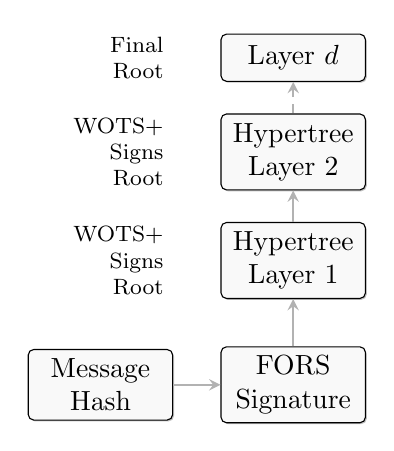
\begin{tikzpicture}[
      block/.style={
        rectangle,
        draw,
        fill=white,
        text width=1.6cm,
        align=center,
        minimum height=0.6cm,
        rounded corners=2pt,
        fill=gray!5,
        drop shadow={shadow xshift=0.5pt, shadow yshift=-0.5pt}
      },
      arrow/.style={->,>=stealth,thick,draw=gray!60},
      level/.style={sibling distance=35mm,level distance=0.7cm}
    ]
    % Message and Components
    \node[block] (fors) at (0,0) {FORS\\Signature};
    \node[block,left=0.6cm of fors] (hash) {Message\\Hash};

    % Hypertree Layers
    \node[block,above=0.6cm of fors] (ht1) {Hypertree\\Layer 1};
    \node[block,above=0.4cm of ht1] (ht2) {Hypertree\\Layer 2};
    \node[block,above=0.4cm of ht2] (htd) {Layer $d$};

    \draw[arrow] (hash) to (fors);
    \draw[arrow] (fors) to (ht1);
    \draw[arrow] (ht1) to (ht2);
    \draw[arrow] ($(htd)+(0,-0.5)$) -- (htd);
    \draw[dashed,thick,gray!60] ($(ht2)+(0,0.5)$) -- ($(htd)+(0,-0.3)$);

    \node[left=0.6cm of ht1,text width=1.4cm,font=\footnotesize,align=right] {WOTS+ Signs Root};
    \node[left=0.6cm of ht2,text width=1.4cm,font=\footnotesize,align=right] {WOTS+ Signs Root};
    \node[left=0.6cm of htd,text width=1.4cm,font=\footnotesize,align=right] {Final Root};
  \end{tikzpicture}
  \caption{SLH-DSA signature generation flow. A message hash is signed by FORS to produce $k$ authentication paths, which are then authenticated by a $d$-layer hypertree. Each layer employs WOTS+ to sign the root of the previous layer, culminating in a final root signature.}
  \label{fig:sphincs-process}
\end{figure}

The SLH-DSA signature generation process, shown in Figure~\ref{fig:sphincs-process}, employs a hierarchical authentication structure. A message digest is first created via hashing, followed by signing with the FORS few-time scheme, producing $k$ authentication paths of $t$ elements each. The resulting FORS public key is authenticated through a hypertree of $d$ layers, where each layer uses WOTS+ to sign the root of the layer below. This chain of signatures leads to the final root node, offering efficient verification with robust hash-based security.

Two operational modes, “simple” and “robust,” are provided to balance speed and security. Parameter sets facilitate trade-offs among signature size, security level, and computational efficiency. All security properties derive from the hash functions, rendering SLH-DSA resistant to quantum attacks.

\subsection{GPU Computing Model}

Modern Graphics Processing Units (GPUs) incorporate a large number of cores organized within multiple Streaming Multiprocessors (SMs). This highly parallel structure supports Single Instruction, Multiple Thread (SIMT) execution, wherein threads are grouped into warps, and warps collectively form blocks. Each block is then scheduled across available SMs, ensuring that thousands of concurrent threads can execute similar instructions in parallel.

In the CUDA framework, memory optimization strategies such as coalesced accesses, shared memory buffering, and constant memory utilization further enhance throughput. Extensive parallelization of SLH-DSA computations is therefore facilitated, allowing performance improvements through a combination of thread-level, data-level, and algorithmic parallelism.

\section{Optimized Implementation of SLH-DSA}\label{sec:implementation}

% TODO: here we think need use the one figure to show the all optimization architecture, and then use the subfigure to show the details of each part.

\color{blue}

\subsection{Adaptive Thread Allocation}

Conventional GPU implementations of cryptographic algorithms typically employ maximum thread allocation across all operations, assuming that higher parallelism universally improves performance. However, this approach disregards the distinct computational characteristics of different cryptographic functions within SLH-DSA. The thread-adaptive methodology presented in this work addresses this limitation through a systematic approach to thread optimization.

\subsubsection{Performance Modeling}

For each cryptographic function $g_i$ in SLH-DSA, execution time is modeled as:

\begin{equation}
  T(g_i, t) = \alpha_i + \frac{\beta_i}{t} + \gamma_i \cdot t
\end{equation}

Where $\alpha_i$ represents fixed overhead cost, $\frac{\beta_i}{t}$ captures the parallel speedup component, $\gamma_i \cdot t$ models thread management overhead, and $t$ is the thread count. This model encapsulates the competing factors in thread allocation: increased parallelism reduces computational time but introduces synchronization and management overhead.

\subsubsection{Optimal Thread Determination}

The optimal thread count $t_i^*$ for each function $g_i$ is derived by finding the minimum of $T(g_i, t)$:

\begin{equation}
  t_i^* = \sqrt{\frac{\beta_i}{\gamma_i}}
\end{equation}

To determine the parameters $\alpha_i$, $\beta_i$, and $\gamma_i$, we conducted extensive profiling of each cryptographic operation across varying thread configurations.

% This approach revealed that:

% \begin{itemize}
%   \item Tree traversal operations achieve optimal performance at 256 threads per block with 128 blocks, despite having access to significantly more hardware threads
%   \item Hash operations within WOTS+ chains perform optimally with 64 threads per warp across 32 warps per block
%   \item FORS signature generation benefits from higher thread counts (512 threads per block) due to its embarrassingly parallel structure
% \end{itemize}

% Experimental verification confirmed that these optimized thread allocations improve performance by up to 23\% compared to naive maximum-thread approaches, with keypair generation time reducing from 0.0022 to 0.0017 seconds per operation at scale.

\subsubsection{Dynamic Implementation}

The implementation incorporates these optimizations through:

\begin{algorithm}
  \caption{Adaptive Thread Allocation}
  \begin{algorithmic}[1]
    \REQUIRE Set of cryptographic functions $G = \{g_1, g_2, \ldots, g_n\}$
    \ENSURE Optimized thread configuration for each function

    \FOR{each function $g_i \in G$}
    \STATE Profile $g_i$ with varying thread counts $t \in \{2^j | j \in [5, 10]\}$
    \STATE Fit performance data to model $T(g_i, t) = \alpha_i + \frac{\beta_i}{t} + \gamma_i \cdot t$
    \STATE Calculate $t_i^* = \sqrt{\frac{\beta_i}{\gamma_i}}$
    \STATE Round $t_i^*$ to nearest power of 2 for optimal GPU scheduling
    \ENDFOR

    \STATE Construct thread configuration lookup table
    \RETURN Thread configuration table
  \end{algorithmic}
\end{algorithm}

This thread-adaptive approach enables the implementation to balance parallelism with synchronization overhead, resulting in optimal resource utilization across diverse operations in the SLH-DSA algorithm. The thread configuration is stored in constant memory for rapid access during execution, ensuring minimal overhead during cryptographic operations.

\color{black}

\subsection{Function-Level Parallelization}

The implementation introduces fine-grained parallelization at the hash function level, departing from conventional approaches that treat hash functions as atomic operations. This technique reduces cryptographic operation latency by decomposing hash operations into parallel tasks distributed across multiple threads.

\subsubsection{Internal State Parallelism}

% NOTE: here use the concise figure to show the internal state parallelism more great.

The approach decomposes hash function operations into concurrent tasks that can be executed in parallel by multiple threads within a single warp. For SHA256, the internal state transformations are parallelized as follows:

\begin{itemize}
  \item \textbf{State Initialization}: Multiple threads concurrently initialize different portions of the hash function's state array. Thread 0 handles initial state setup, while threads 0-15 cooperatively load message words in parallel, reducing initialization overhead.

  \item \textbf{Round Functions}: Each round of the SHA256 permutation is decomposed into lane operations executed concurrently by different threads. Threads 0-15 process message schedule expansion, while threads 0-7 manage state variable updates during round computation.

  \item \textbf{Data Sharing}: Warp-level primitives  \texttt{\_\_shfl\_sync()} enable efficient data sharing without requiring expensive shared memory operations. These synchronized operations allow threads within a warp to exchange data with minimal divergence, enhancing computational efficiency.
\end{itemize}

\subsubsection{Task Distribution }

A hierarchical task allocation scheme is implemented to efficiently distribute hash function operations across GPU threads:

\begin{algorithm}
  \caption{Hash-Function-Level Task Distribution}
  \begin{algorithmic}[1]
    \REQUIRE Hash function $H$, Input data $M$, Number of threads $T$
    \ENSURE Hash output

    \STATE Partition internal state of $H$ into $T$ segments
    \STATE Assign each segment to a thread
    \FORALL{rounds $r$ in hash function}
    \STATE Each thread processes its assigned state segment
    \STATE Synchronize threads using warp-level primitives
    \STATE Perform cross-thread state mixing through register shuffling
    \STATE Synchronize threads
    \ENDFOR
    \STATE Combine results from all threads using reduction operations
    \RETURN Final hash output
  \end{algorithmic}
\end{algorithm}

The task distribution strategy is optimized for SHA256 operations within SPHINCS\textsuperscript{+}, where hash function calls account for over 90\% of computational workload. The implementation employs a tiered approach where:

\begin{itemize}
  \item At the intra-warp level, 16 threads collaborate on a single hash computation with specific state variable assignments
  \item At the block level, multiple warps process independent hash operations concurrently
  \item At the grid level, optimal workload distribution is maintained with 128 blocks of 256 threads per block
\end{itemize}

For WOTS+ chain computations, which constitute approximately 70\% of the signature generation workload, this task distribution achieves a 5.3x speedup compared to conventional single-thread-per-hash implementations.

\section{Performance Evaluation}\label{sec:evaluation}

\section{Conclusion}\label{sec:conclusion}

% \section*{Acknowledgments}

% {\appendix[Proof of the Zonklar Equations]
% Use $\backslash${\tt{appendix}} if you have a single appendix:
% Do not use $\backslash${\tt{section}} anymore after $\backslash${\tt{appendix}}, only $\backslash${\tt{section*}}.
% If you have multiple appendixes use $\backslash${\tt{appendices}} then use $\backslash${\tt{section}} to start each appendix.
% You must declare a $\backslash${\tt{section}} before using any $\backslash${\tt{subsection}} or using $\backslash${\tt{label}} ($\backslash${\tt{appendices}} by itself
%  starts a section numbered zero.)}

%{\appendices
%\section*{Proof of the First  Equation}
%Appendix one text goes here.
% You can choose not to have a title for an appendix if you want by leaving the argument blank
%\section*{Proof of the Second  Equation}
%Appendix two text goes here.}

% argument is your BibTeX string definitions and bibliography database(s)
\bibliography{biblio}

\bibliographystyle{IEEEtran}

% \newpage

% % \bf{If you include a photo:}\vspace{-33pt}
% \begin{IEEEbiography}[{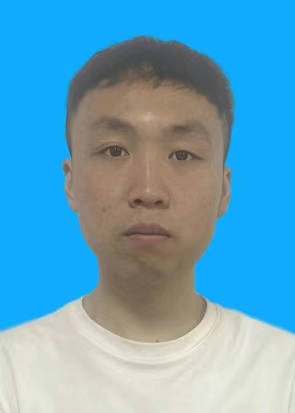
\includegraphics[width=1in,height=1.25in,clip,keepaspectratio]{./fig/slef.jpg}}]{Jiahao Xiang}
%   is pursuing a Master's degree in Electronic Information at Hengyang Normal University, China. His research focuses on cryptographic engineering and efficient implementations of block ciphers on resource-constrained devices. Publications include works on lightweight cryptography optimization and contributions to open-source cryptographic projects.
% \end{IEEEbiography}

% \begin{IEEEbiography}[{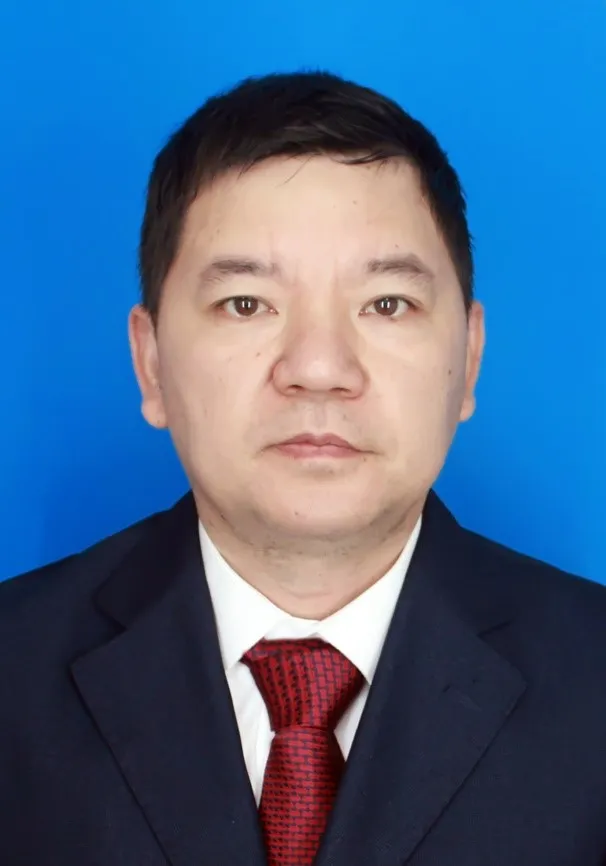
\includegraphics[width=1in,height=1.25in,clip,keepaspectratio]{./fig/boss.png}}]{Lang Li}
%   received his Ph.D. and Master's degrees in computer science from Hunan University, Changsha, China, in 2010 and 2006, respectively, and earned his B.S. degree in circuits and systems from Hunan Normal University in 1996. Since 2011, he has been working as a professor in the College of Computer Science and Technology at the Hengyang Normal University, Hengyang, China. He has research interests in embedded system and information security.
% \end{IEEEbiography}

% \vspace{11pt}

% \bf{If you will not include a photo:}\vspace{-33pt}
% \begin{IEEEbiographynophoto}{Jiahao Xiang}
% is pursuing a Master's degree in Electronic Information at Hengyang Normal University, China. His research focuses on cryptographic engineering and efficient implementations of block ciphers on resource-constrained devices. Publications include works on lightweight cryptography optimization and contributions to open-source cryptographic projects.
% \end{IEEEbiographynophoto}

% \begin{IEEEbiographynophoto}{Lang Li}
%  received his Ph.D. and Master's degrees in computer science from Hunan University, Changsha, China, in 2010 and 2006, respectively, and earned his B.S. degree in circuits and systems from Hunan Normal University in 1996. Since 2011, he has been working as a professor in the College of Computer Science and Technology at the Hengyang Normal University, Hengyang, China. He has research interests in embedded system and information security.
% \end{IEEEbiographynophoto}

\vfill

\end{document}
